\documentclass{article}
\usepackage[utf8]{inputenc}
\usepackage[margin=0.75in]{geometry}
\usepackage{cite}
\usepackage{colortbl}
\usepackage{booktabs}% http://ctan.org/pkg/booktabs
\newcommand{\tabitem}{~~\llap{\textbullet}~~}
\usepackage[hidelinks]{hyperref}
\usepackage{subcaption}
\usepackage{graphicx}
\usepackage{titlesec}% http://ctan.org/pkg/titlesec
\titleformat{\section}%
    [hang]% <shape>
    {\normalfont\bfseries\Large}% <format>
    {}% <label>
    {0pt}% <sep>
    {}% <before code>
\renewcommand{\thesection}{}% Remove section references...
\renewcommand{\thesubsection}{\arabic{subsection}}%... from subsections
\usepackage{bookmark}
\usepackage{enumitem}
\usepackage{multicol}
\usepackage[figuresleft]{rotating}

\begin{document}
\begin{center}

    % MAKE SURE YOU TAKE OUT THE SQUARE BRACKETS

    \LARGE{\textbf{COMP 3004 - Deliverable \#3 \\ System Architecture and Design}}\\ 
    % \vspace{1em}
    \Large{\href{https://github.com/alextrosta/brackit}{\texttt{Brackit}} - Mobile Tournament Bracket Creation} 
    % \vspace{1em}
    % \normalsize\textbf{Jaime Herzog, Suohong Liu, Xiyi Liu, Alex Trostanovsky} \\
    % \normalsize{
    %     \href{mailto:jaime.herzog@carleton.ca}{jaime.herzog@carleton.ca},
    %     \href{mailto:suohong.liu@carleton.ca}{suohong.liu@carleton.ca},
    %     \href{mailto:xiyi.liu@carleton.ca}{xiyi.liu@carleton.ca},
    %     \href{mailto:alex.trostanovsky@carleton.ca}{alex.trostanovsky@carleton.ca}
    % }\\
    % \normalsize{
    %     101009321,
    %     101002340,
    %     101004577,
    %     100984702,
    % }
    % \vspace{1em}
    % \normalsize{Carleton University, School of Computer Science} \\
\end{center}
% \begin{normalsize}

% \end{normalsize}

\section*{Metadata}
\subsection*{Team / App Name: \href{https://github.com/alextrosta/brackit}{\texttt{Brackit}}}
% \textbf{Team Member Names:}\\ Jaime Herzog: 101009321, Suohong Liu: 101002340, Xiyi Liu: 101004577, Alex Trostanovsky: 100984702


\subsection*{Team member names}
\begin{center}
    \begin{tabular}{ |l|c| }
        \hline
        \textbf{Name}     & \textbf{Student ID} \\
        \hline
        Jaime Herzog      & 101009321           \\
        Suohong Liu       & 101002340           \\
        Xiyi Liu          & 101004577           \\
        Alex Trostanovsky & 100984702           \\
        \hline
    \end{tabular}
\end{center}
\tableofcontents
\clearpage
\section{Architecture}
% identify, describe, and justify the architecture of your project (architectural style, design patterns) \\
% Outcome is a system architecture that supports the functional goals and non-functional attributes of your project 
\subsection{Description}
In developing \texttt{Brackit}, we set out to address an urgent need by tournament attendants and organizers to visualize, manage, and interact with double elimination
brackets on their mobile devices. At a high level, we committed to developing a product that will meet the following \textbf{functional requirements}:
\begin{enumerate}
    \item{Tournament Organizers (TO's) can create, host, maintain, and visualize double elimination brackets.}
    \item{Registerd \texttt{Brackit} Users, as well as Guests, can use the application to join created tournaments.}
    \item{\texttt{Brackit} will store and maintain user profiles that will describe users' history:
    \begin{itemize}
        \item{Matches won/lost}
        \item{Tournaments entered/created}
    \end{itemize}
    }
\end{enumerate}
In terms of \textbf{non-functional requirements}, we believed \texttt{Brackit} be \textit{usable} on mobile devices. \texttt{Brackit} users should be able to:
\begin{itemize}
    \item{View and access all submodules (Brackets, Rounds, Matches) of a tournament on an Android device}
    \item{Seamlessly enter tournament competitors to brackets on an Android device}
\end{itemize}

Conceptually, \texttt{Brackit} needed to support the creation and maintenance of the following \textit{components}:
\begin{itemize}
    \item{\textit{Tournament}: The highest level abstraction utilized in Bracket creation. A tournament acts a \textit{container} for brackets.}
    \item{\textit{Bracket}: Given the number of entrants and their corresponding seeds (ranks), 
    Double elimination brackets dictate competitor matchups and the progression of competitors through the Winners and Losers brackets }
    
\end{itemize}  
\subsection{Justification}
To deve
\clearpage
\subsection{Architectural Diagrams}
\vfill
\begin{center}
    \begin{figure}[htp]
        \centering
        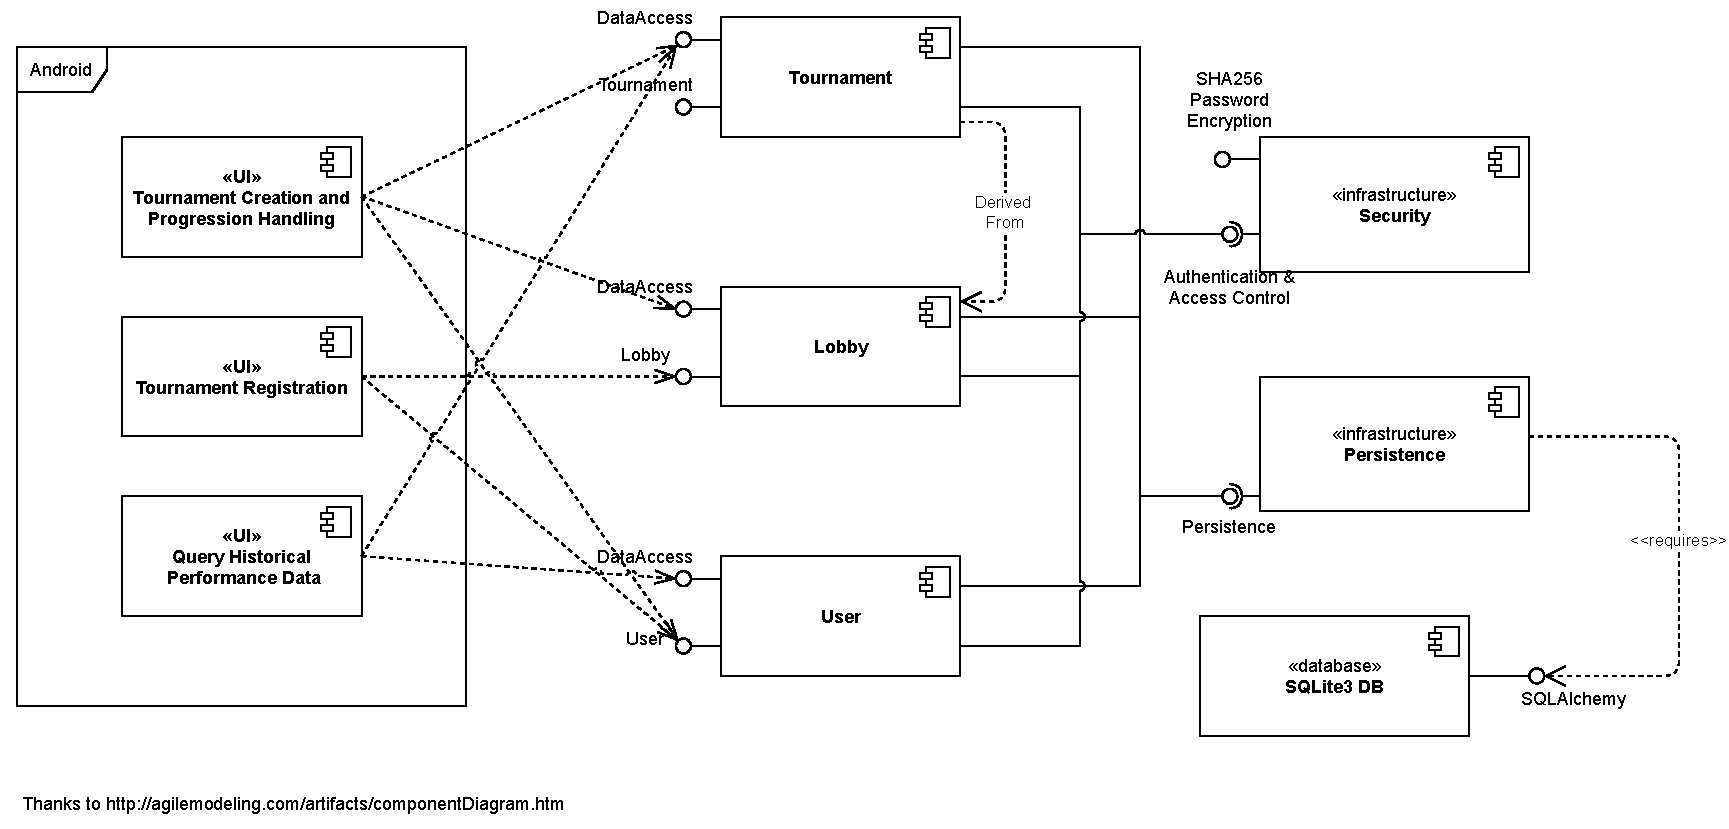
\includegraphics[width=18cm]{../diagrams/component_diag.pdf}
        \caption{\texttt{Brackit - }\href{https://sparxsystems.com/resources/tutorials/uml2/index.html}{UML 2} Architectural Component Diagram}
        \end{figure}
\end{center}
\vfill

\begin{center}
    \begin{figure}[h]
        \centering
        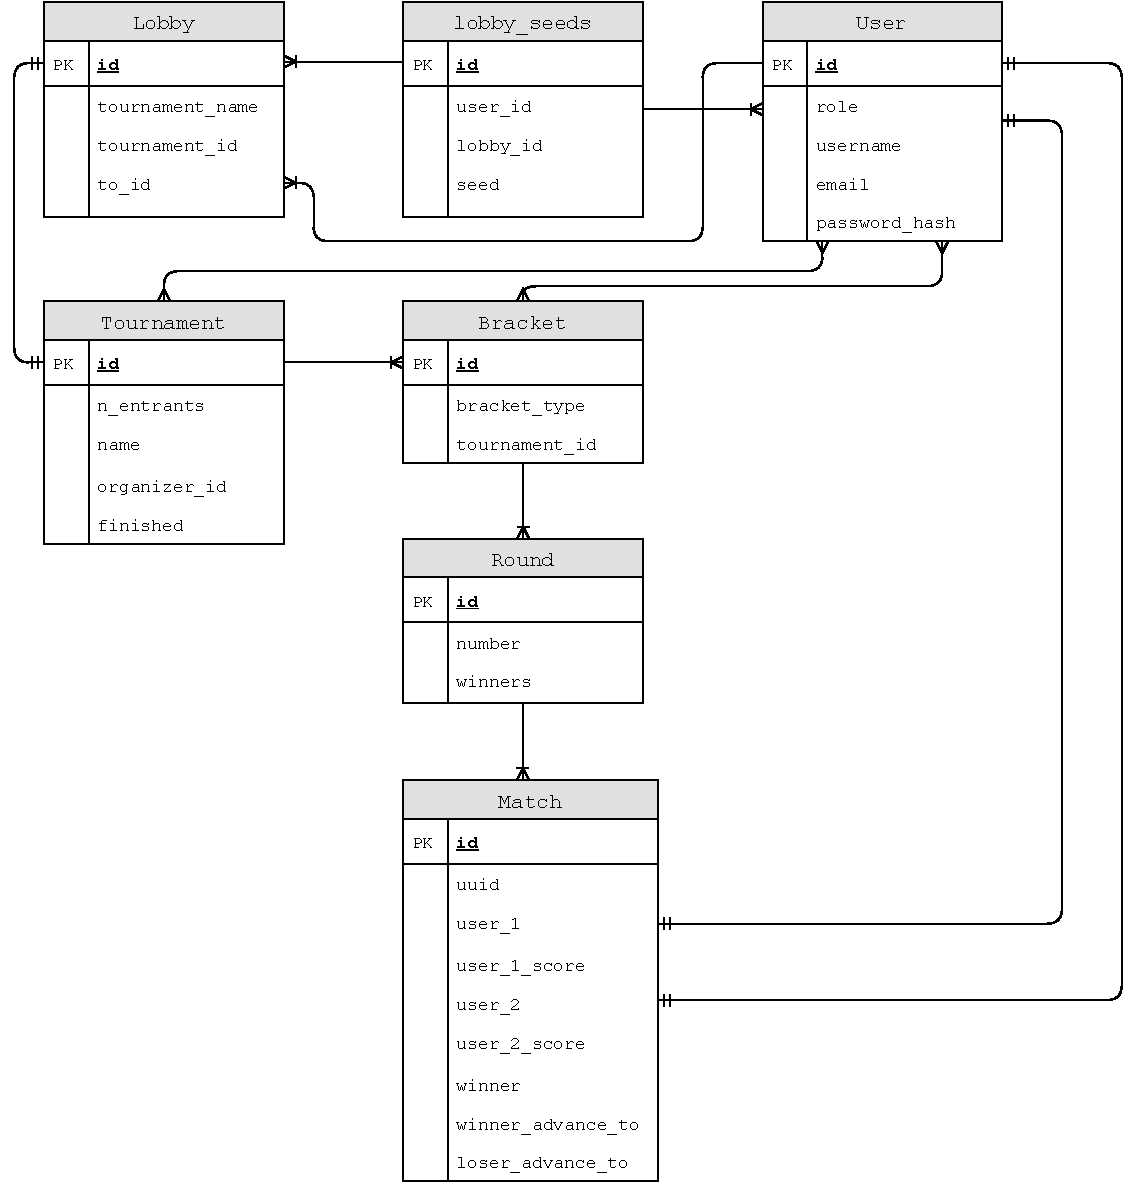
\includegraphics[width=19cm]{../diagrams/er.pdf}
        \caption{\texttt{Brackit - } Entity Relationship (ER) Diagram}
        \end{figure}
\end{center}
\clearpage
\section{Design}
\subsection{Description and Rationalization}
The Brackit backend was designed primarily to marry extensibility with the correctness of 
our relatively complex domain. The main challenge of the backend's design is the creation of 
correct brackets, as well as the maintenance of brackets as they progress to completion.

When we create a Tournament, we create a tournament object in the backend, which itself creates
the bracket. Depending on the bracket type, it creates the appropriate number of rounds, 
with each round having its appropriate number of matches. This is handled automatically because
the number of rounds is deterministic to the number of entrants and the type of bracket. See the discussion
on the justification of the object-oriented architecture.
So far, we only have the double elimination bracket type implemented, but this can be expanded easily by just adding additional 
cases in the Bracket constructor. An alternative approach would be to create an abstract Bracket
class with each bracket type as an implementation of the abstract Bracket class. This may allow for 
code that is easier to read and iterate on, and would be worth the time spent refactoring if this project were 
to be expanded on.

A specific implementation challenge is hangling how each match knows who is the entrant which is playing 
in said match. This is called progression - for matches in the initial rounds, this is trivial as 
the entrants are simply placed into the matches when the Tournament is instantiated, but as the tournament
progresses, 

Our backend uses the Flask python package to expose our bracket and user information to 
the frontend, as well as SQLAlchemy to manage our information in the database. SQLAlchemy has a 
Model package which models our objects in the table, and provides the interface from which we interact
with our database at runtime. We model each class in our class diagram in models.py, which creates 
tables for each class and defines the table relationships in an object oriented style. This 
allows us to query the database itself easily and safely when the APIs are invoked, enabling 
easy retrieval of the specific object being requested. Additionally, these models allow for 
easy sql querying for user data, such as users cross-tournament wins and losses. 

\subsection{Design Patterns}
\begin{enumerate}
    \item Facade Pattern
    
    The Facade pattern intends to provide a unified interface to a set of interfaces in a subsystem. 
    For our backend, the API endpoints contained in the routes.py constitute our Facade,
    as each endpoint provides a centralized and easy to use endpoint which the user can access
    and which invokes all necessary interfaces to execute the necessary code in the backend.

    This pattern facilitates a single way in which frontend clients can access backend data,
    as well as centralizes all exposed endpoints on the server side, allowing for ease of
    extensibility.

    \item Singleton Pattern 
    
    The Singleton pattern intends to ensure a class has only one instance, and to allow global 
    access to that class. The Flask app object leverages the Singleton pattern in its design, as 
    it is instantiated only once when the server is started, and is accessed globally throughout the 
    backend. 

    The justification for the use of the Singleton pattern for the app object is because the app 
    class itself, when instantiated, is the representation of the Flask server instance at compile time,
    and is how we modify and customize our server, i.e. specifying the database schema, or specifying the API 
    endpoints. Additionally, ensuring the app is only instantiated once maintains consistency throughout the session,
    as multiple apps could potentially create multiple duplicate endpoints, which would create unintentional behaviour
    such as method invokation duplication.
\end{enumerate}
\clearpage
\section{Design Diagrams}
\begin{center}
    \begin{figure}[htp]
        \centering
        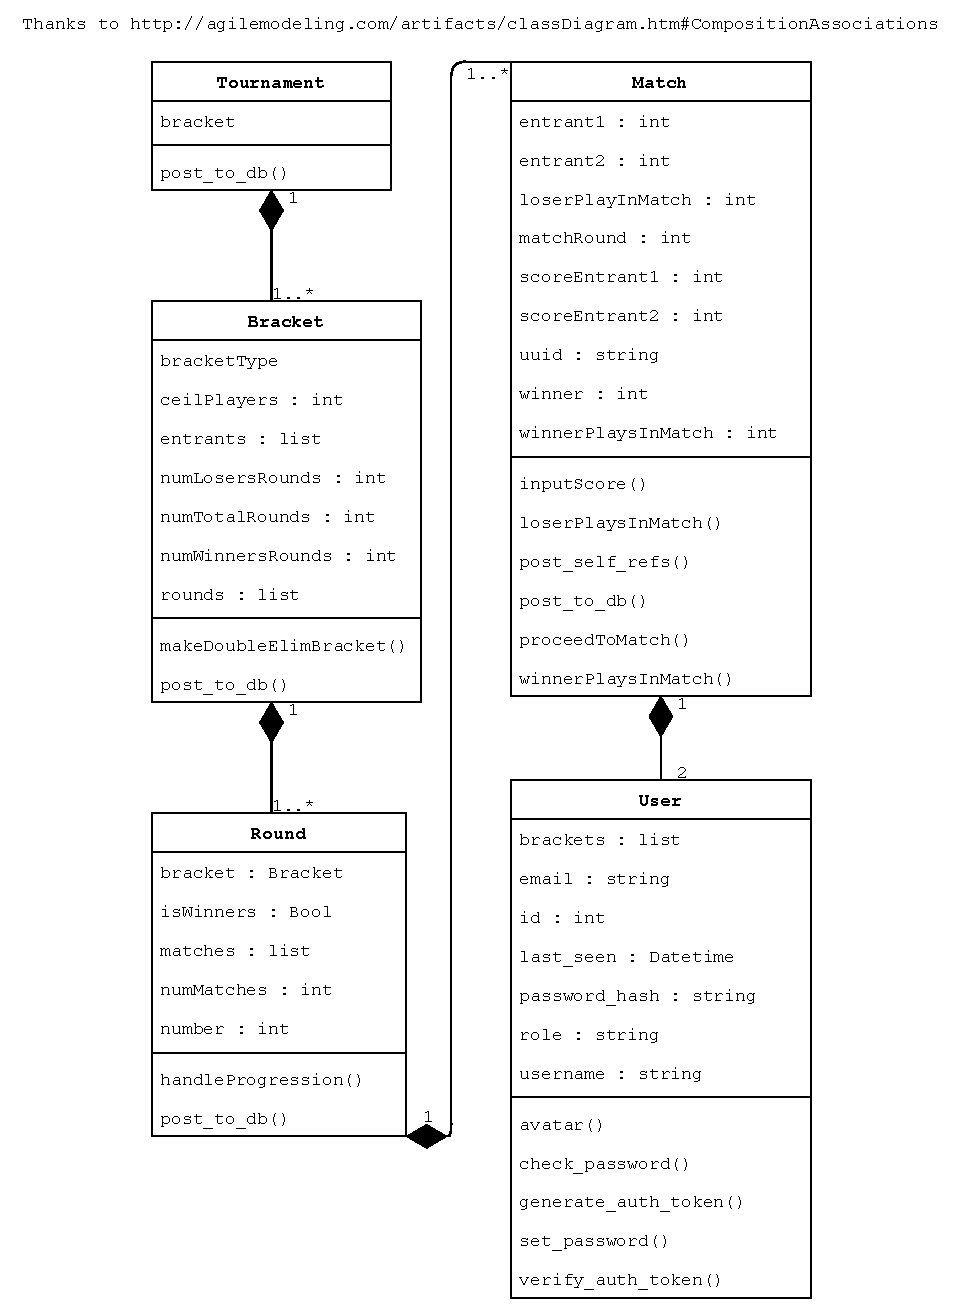
\includegraphics[width=13cm]{../diagrams/uml_class_tourn.pdf}
        \caption{\texttt{Brackit - }UML Class Diagram}
        \end{figure}
\end{center}



\clearpage
%\cite{wiki:xxx}
%\bibliographystyle{unsrt}
%\bibliography{ref.bib}


\end{document}